% chap2.tex {Background}
\newpage
\thispagestyle{empty}
\mbox{}


\chapter{Background}\label{BACK-CHAP}
This chapter presents a brief description of all technologies, strategies, and frameworks used to develop and run the testbed. Section \ref{sec:nta} talks about different networking testing approaches and its advantages and disadvantages. Section \ref{sec:sdn} introduces SDN architecture along with important aspects of the OpenFlow protocol and gives a brief overview of Open vSwitch. Section \ref{sec:fcpf} discusses FCAPP, its problem statement, and the approach followed to solve the problem. Lastly, Section \ref{sec:tools} introduces all the tools and technologies used in the testbed and the justification for using them.

\section{Network Testing Approaches}\label{sec:nta}
There are four general approaches that are often used for testing computer communication network applications. These are mathematical analysis, simulation, emulation, and a real network testbed \cite{doi:10.1287/opre.50.1.125.17772} \cite{Krop:2007:JCS:1287767.1287774}. Each method has its advantages and disadvantages and is appropriate at a different time of development cycle. 

Only general ideas come up during the initial phase of the design, such as the behavior and reaction of the application in certain situations. With these ideas, a model of the application can be developed. A mathematical analysis is capable of evaluating the feasibility and performance of an experimental model. If the model's performance is promising, an actual implementation might be developed. The implementation describes how the application would respond in every possible situation. Simulation, emulation and real network testbeds are used to evaluate the implementation to see if it performs as the model suggested.

\subsection{Mathematical Analysis}
Mathematical analysis usually reproduces the network by using stochastic queuing models \cite{2013arXiv1307.2968Z} to determine how the network would perform in certain situations. These models require various assumptions to be made in order to perform evaluation and analysis. Even with these assumptions, it can become very lengthy and complicated. Simulation is usually used as an alternative to mathematical analysis.

\subsection{Network Simulations}
Most network simulators use a discrete event-based approach to modeling network operation. In this approach, the network represented by a collection of nodes (e.g., switch and router) and edges (e.g., links) as in a graph and the operation is reproduced as a collection of events. An example of key events that a simulator would keep track of would be a traffic flow generation or processing of the flow by an application. These key events are typically stored in a list and sorted by the time at which the event was executed (e.g., the flow generation). The list is then traversed and executes each event in sequential order. Normally, simulation approaches use an artificial representation of time. The current time in the simulation is given by the time of the event being executed. If there is no event during a given period of time, then the simulation can skip over this time as being unimportant. Additionally, some events might take a long time to be executed, but this does not matter to the simulator since the representation of time is artificial and does not have to be synchronized with an outside clock. Therefore, the length of simulation is dependent on the complexity of the application and the amount of traffic, and not on the length of time it would take to execute in real time. To illustrate, if a researcher wanted to model a scenario with thousands of flow over a network consisting of hundred nodes for 24 hours, that simulation might only take a few minutes to evaluate. In a real situation, one has to wait for 24 hours to evaluate the result. In the simulation, the reproducibility of results for later statistical analysis is guaranteed. This is often not possible in real world experiments due to many unpredictable impacts. Simulations usually only require one computer to perform the desired analysis. This means that simulations allow a cost-efficient way of researching complex systems. However, the difficult part of using a computer simulation is creating a representative implementation of the original system in a model. Additionally, to cope with the real system's complexity, the simulation model requires abstractions and simplifications, which possibly do not have an impact on the final result.

\subsection{Network Emulations}
Emulation is a technique to provide the interface and functionality of a system component in a potentially unrelated environment. In the best case, emulation offers the same functional (service) and non-functional properties (performance) as the original system. Since an emulation imitates the real system that it models, it can be used transparently without requiring many changes in the real setup. The target network environment in emulation can be reproduced by means of a virtualization mechanism. For example, when sending packets, the actual protocol and application implementation is used, but links that the packet travels over are modeled. This is done by imposing additional delays, and by restricting the bandwidth of the laboratory network to more closely reflect the network being emulated. It allows running the original protocols and applications of a real OS (Operating System). Since the actual application implementations are used, the emulator must be executed in real time, so that the application's behavior does not have to be modified. This makes network emulation a valuable technique to study realistic network scenarios \cite{Zheng2012}. Additionally, emulation usually involves multiple computers, mostly employing a one to one mapping scheme between nodes in a real situation and virtual node used in the emulation. This one to one mapping scheme has serious implications on scalability, that means the hardware setup in the laboratory has to be relatively large to accommodate all the nodes. The benefit of emulation is that the network links are modeled, allowing for ad hoc and distributed networks to be evaluated in a cost-effective manner. Additionally, an emulator can be easily reconfigured, because no hardware needs to be manipulated to make changes to the emulated network. Furthermore, emulation results usually can be reproduced over multiple runs, which aids in the debugging of the application \cite{Noble:1997:TMN:263109.263140} \cite{Lochin2012}.

The authors of \cite{eoeqofohn} provided a detailed discussion of this topic. There are mainly four major application areas for network emulation, as follows: 
\begin{itemize}
	\item Examination of a protocol implementation under different network scenario and detect its limitations, error or external effects, and problems,
	\item Examination of different protocols using the same network and traffic load conditions to study the advantages and disadvantages of them,
	\item Evaluation of protocols and network applications for performance benchmarking, and 
	\item Analyzation of the effectiveness of distributed network applications in a real network scenario.
\end{itemize}

Network emulation is an ongoing field of research in which a number of different approaches have been developed to reproduce a target network environment, where the target network is the network to which the protocol or application is designed to be used on. However, all of these approaches have some general characteristics in common. These characteristics include:

\begin{itemize}
	\item Actual protocol implementation - the actual implementation of the protocol or application should be used,
	\item Real traffic - packets should be transmitted between nodes,
	\item Real time - the testing should be conducted in the same amount of time that the application would normally take so that the application's performance can be accurately measured, and
	\item Network links modeled - the links between the nodes in the laboratory should be augmented so that they appear like links in the target network and not like the physical links in the laboratory. This also allows for the topology of the target network to be changed without making any modifications to the hardware in the laboratory.
\end{itemize}

Most emulation approaches use the same basic architecture consisting of applications (for traffic generating or receiving) and a network description. The network description consists of the location of the nodes, relevant hardware information (e.g., CPU power, memory), and the characteristics of the links (e.g., delay, bandwidth), also called the network model. The network model is then passed to a traffic shaper which applies the link characteristics to packets sent over the network by the application. The traffic shaper is usually implemented in the kernel of the operating system. This structure is illustrated in Figure \ref{fig:emulator} and followed by the definitions of the different elements.

\begin{figure}[H]
\begin{center}
	{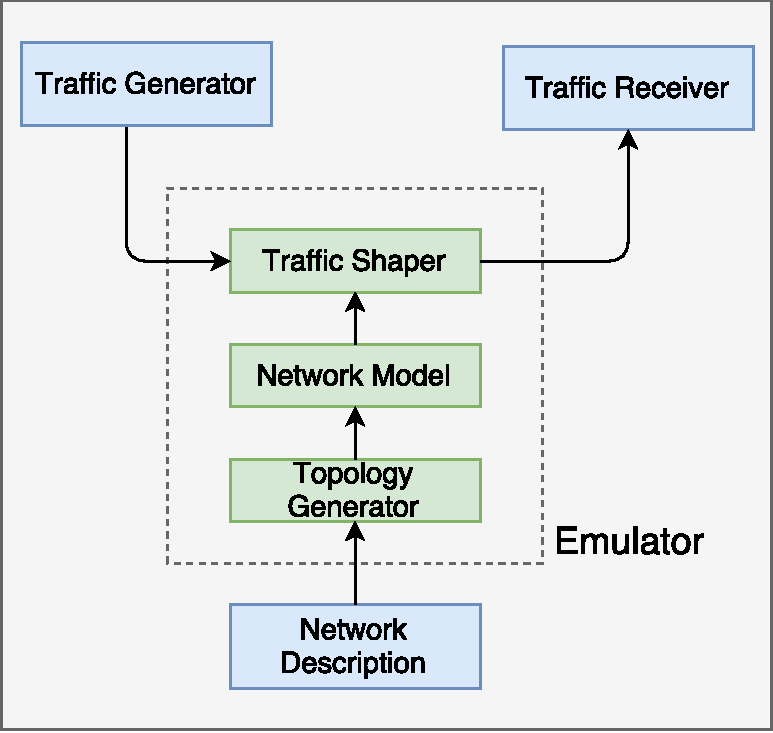
\includegraphics[width=0.5\textwidth]{emulator.pdf}}
	\caption{Basic structure of emulation}
	\label{fig:emulator}
\end{center}
\end{figure}

Definitions of the building blocks of emulation:
\begin{itemize}
	\item Application - here applications are the traffic generator or traffic receiver.
	\item Traffic Shaper - this is normally an operating system process which applies the physical properties (e.g., delay, bandwidth) of the target link in software. The traffic shaper must work in real time.
	\item Network Description - information about the nodes in the network, including position and relevant hardware information, along with the link description.
	\item Topology Generator - the topology generator translates the network description into a model of the network nodes and links.
	\item Network Model - a real-time description of the network nodes and links, including information about which links between which nodes are available and their characteristics (e.g., delay, bandwidth).
\end{itemize}

These are the basic elements of an emulator even though most emulators do not make a clear distinction between the different elements. This allows for a two-stage approach \cite{Perennou2005}, where the network description is converted to a network model in the first stage, and then the traffic shaper is applied on the network model in the second stage. This approach can be beneficial because the first stage does not have to be done in real time, so the computations can be more complex, allowing for more complicated phenomena to be considered. However, in the second stage, the application of the network model must still be done in real time.

\subsection{Real Network Testbeds}
Real network test beds use the actual implementation, along with the actual network links, to determine the performance of a network. This means that the test will be executed in real time, just as it would in real life scenario. Additionally, since the links are the actual physical links that would be used in real life, the results produced by a real network testbed would be an extremely accurate depiction of how the network would actually perform. The drawback to this approach is that it is very expensive and sometimes impossible to reconstruct. Every node in the scenario and the links connecting the nodes together has to be the same links that would be used in the actual network. For large mobile networks, this can be a very difficult task to faithfully represent it and the motion of the user device would have to be precisely reproduced. Even if the motion can be reproduced, the interference encountered by the nodes would have to be reproduced which might be difficult to attain \cite{Noble:1997:TMN:263109.263140}. Real network testbeds are also not very flexible since hardware changes must be made to create a different scenario. This forces the researcher to only consider a subset of the possible networks on which the application could be deployed.

\section{Software-Defined Network}\label{sec:sdn}
Software-Defined Networking (SDN) is an emerging concept that is dynamic, manageable, cost-effective, and adaptable, making it ideal for the high-bandwidth, dynamic nature of today's applications \cite{sdn-def}. Fundamentally, the SDN concept separates the network data plane, i.e., the network devices that forward traffic, from the control plane, i.e., the software logic that controls ultimately how traffic is forwarded through the network. The separation of the network's data plane and control plane allows the network operator to control network behavior from a single high-level control program. The main goal of SDN is to make the network more open and programmable. If an organization requires a specific type of network behavior, it can develop or install an application to do what it needs to do. These applications may be for networking functions, e.g., traffic engineering and security. There can also be applications for functionality that have not been thought of today and will be introduced in the future. This kind of flexibility would allow the network to evolve at the speed of the software. A desktop computer operating system model can be broken down to understand the SDN model. 

A desktop computer OS has three basic layers. First, there is the operating system itself that manages access of applications to underlying hardware. The OS also comes with core services to aid, i.e., responsible for managing system hardware on the lower level, e.g., CPU, storage, memory, and network interfaces. It can also be called the south of the OS instead of the lower level. Above the operating system, on the north side, are the applications. The ability to develop or add and remove applications makes the system a flexible one that can be customized to the costumers' specific needs whether gaming, design, engineering, and so on.

The SDN model also looks quite similar to the operating system model. In SDN, there is a network operating system or NOS instead of the operating system in the middle layer. This is also commonly called an SDN controller. The network operating system will typically have core services to aid in its job such as interfacing with network nodes and providing a programmable interface to the network applications. On the south side, instead of a hardware like a processor, storage, and memory, there are network forwarding devices that receive packets, take actions on those packets and update counters. The types of actions include simply dropping the packet, modifying packet headers, and sending packets out a single or multiple ports. The instructions on how to handle packets originate from the SDN controller. Like the desktop model on the top of the north side, there are applications, also called network applications, which similar to applications on top of a standard OS, can serve many purposes, but with SDN, are all network focused \cite{6994333}.

\begin{figure}[tb]
\begin{center}
	\resizebox{\textwidth}{!}
	{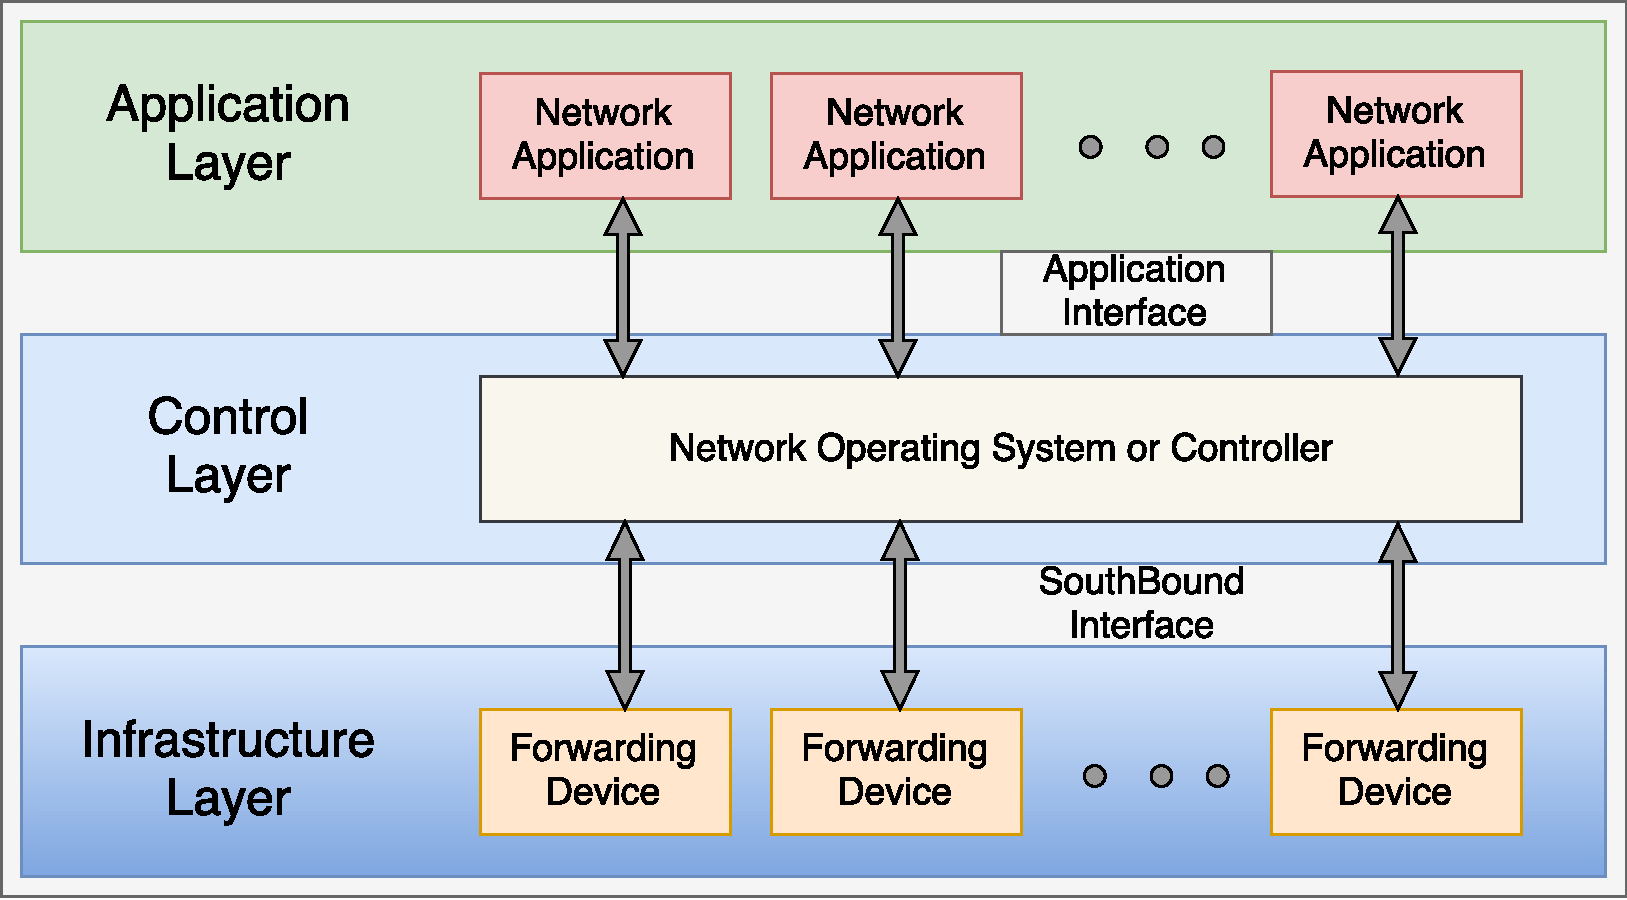
\includegraphics{sdn-architecture.pdf}}
	\caption{SDN architecture \cite{6994333} \cite{sdn-def}}
	\label{fig:sdnarch}
\end{center}
\end{figure}


Figure \ref{fig:sdnarch} provides an overview of the SDN model and its components, which are described in detail below.

\paragraph{Forwarding Devices:}
Forwarding devices, found at the lowest layer, can be conventional hardware switches as long as it support a programmable interface like OpenFlow (see Section \ref{sec:openflow}), or software switches like Open vSwitch (see Section \ref{sec:ovs}). Hardware switches are usually expected to support higher performance while software switches provide greater flexibility for new behaviors.

\paragraph{SouthBound Interface:}
The SDN controller needs a way to communicate with network forwarding devices. The information that needs to be communicated includes packet handling instructions, alerts of packet arrivals on network nodes, notifications of status changes like links going up or down, and statistics information like flow counters. All these happens over the southbound interface. The popular protocol for SDN on the southbound interface is OpenFlow for packet handling instructions. Complimentary to OpenFlow is the Open vSwitch Database Management protocol (OVSDB) \cite{ovsdbproto} which is a network management protocol used to manage network device configurations in Open vSwitch. It is also being adopted by some hardware-based switches.

\paragraph{Network Operating System:}
The network operating system is commonly referred to as an SDN controller. The controller typically runs with key core services, such as topology, inventory, and statistic services, and a host tracker. The topology service determines how forwarding devices are connected to one another and build what is known as a topology graph. For example, this might work by instructing switches to send Link Layer Discovery Protocol (LLDP) packets or other specialized packets and discovering where they arrived. An inventory service is used to track all SDN-enabled devices and record basic information about them, e.g., the version of OpenFlow and capabilities it support. A statistic service can be employed for reading counter information of floating devices like traffic counters on flows interfaces and flow tables. A host tracker discovers where IP address and MAC addresses of hosts are located in the network, typically by intercepting packets in the network or perhaps in coordination with the virtual machine (VM) platform.

\paragraph{Application Interface:}
The SDN controller provides application interfaces for network applications to hook into. It should be able to provide a simplified abstraction of the underlying network infrastructure often sufficient for the entire network fabric to be represented as a single large switch. For an application, there can be native plug-ins co-located with controllers and using a programming language-based application program interface (API) (e.g., Java API). There is a northbound interface as well, commonly a RESTfull interface which allows the use of standard HTTPS calls directed towards the controller to control network behavior and gather information collected by core services.

\paragraph{Network Application:}
Network applications can serve a wide range of disciplines. With SDN providing a programmable abstraction of the network, network applications can effectively be whatever an organization requires it to be in the context of controlling network behavior and implementing network policies.

\paragraph{}
As to how an SDN network works differently compared to today's conventional networks, below are some important concepts \cite{sdn-def}.

\paragraph{Fault tolerance and scalability:}
Commonly, an SDN controller is referred to as being logically centralized. It is important to understand how this is different from being physically centralized. In a production network, no one would depend on a single physical SDN controller. This would lead to a single point of failure for the entire network, and additionally, there could be scaling limitations. There are different ways to ensure that SDN network is both highly available and scalable. One is clustering and teaming, which is not new in areas like database servers. The idea is to have a cluster of systems that can load balanced workload and provide high availability since one or more systems can break down, ensuring there are still active functional systems. This also provides scalability as multiple systems can handle requests. 

Additionally, the network can be separated into different regions with each region's traffic handled by a regional SDN controller. Different regions can then communicate information between one another as needed using an east-west protocol. SDN controllers also might be designed in a hierarchy. There may be high-level controllers with high levels of abstraction and lower level controllers underneath closer to the network forwarding devices \cite{6994333}.

\paragraph{Directly programmable:} This gives the flexibility to network administrators who directly program network control because it is separated from forwarding devices \cite{sdn-def}.

\paragraph{Agile:} Abstraction of the control from forwarding devices allows administrators to dynamically adjust network-wide traffic flow to achieve changing needs of the environment \cite{sdn-def}.

\paragraph{Programmatically configured:}
SDN allows network managers to write dynamic, automated SDN programs to configure, manage, secure, and optimize network resources very quickly \cite{sdn-def}.

\paragraph{Open standards-based and vendor-neutral:} SDN is implemented through open standards-based which simplifies network design and operation. The control instructions are provided by SDN controllers rather than multiple, vendor-specific devices and protocols \cite{sdn-def}.

\paragraph{Conventional Network Devices}
\paragraph{}
In conventional networks, nodes have a data plane and a control plane both contained within a single physical system. The function of the data plane is to handle packets and line rate in hardware based on information stored in tables like the FIB, LFIB and MAC tables. Execution instructions in the data plane originated in the control plane. The control plane is sometimes referred to as the network nodes brain. The network node uses the control plane to communicate with other nodes in the network. They usually run distributed protocols like BGP, MPLS, and OSPF. Thus, the control plane handles the complexity and it is where network policies are enforced. The control plane determines how individual packets should be handled and pushes this information down to the fast path in the hardware-based data plane. 

Different from the SDN ecosystem discussed earlier, conventional network nodes are, first, proprietary locked boxes. Second, the control plane is chained in the data plane and both are coupled together in a single network node. There is no direct access to the behavior of the data plane to implement network policies so that network operators have to think in terms of what is already available in the control plane or what features or options the device include. Operators most often configure the device through a command-line interface. If a new kind of network behavior is required, options can be limited. 

Another disadvantage of a conventional network compared to an SDN network is that each network node has to be configured individually, so the network operator needs to deal with multiple points of configuration. In a data center, for example, there could be tens or hundreds of nodes to reconfigure to implement new policies. Each of these nodes has its own control plane and all these control planes must communicate using distributed protocols. Therefore, this conventional network paradigm is typically complex and can lead to configuration error as cited earlier \cite{6994333}. 

By contrast with SDN, conventional networks have a lengthy vendor equipment product life cycles. It does not have any specific standard and the lack of open interfaces limit the ability of network operators to adapt the network to their individual environment's requirements \cite{sdn-def}. However, it is important to note that significant complexity may be present in the architecture of the SDN controller itself to accomplish all of its benefits.

\subsection{OpenFlow}\label{sec:openflow}
As previously mentioned, OpenFlow is the standard communications interface defined between the control and forwarding layers of an SDN architecture \cite{openflow}. OpenFlow allows direct access to SDN-enabled devices, such as switches and routers, both physical and virtual. In the SDN architecture (see Figure \ref{fig:sdnarch}), business requirements come into play in the control layer. A control layer software figures out how to translate these requirements into commands to the switches and instructs how to route traffic. The OpenFlow protocol conveys that information to the switches and the switches process the traffic as it comes through. Thus, OpenFlow is a standardized protocol for interaction and manipulation of the forwarding plane or network devices such as switches and routers.

\paragraph{Switch Components}
\paragraph{}
Logically, an OpenFlow switch has one or more flow tables and a group table, which are responsible for packet lookups and packet forwarding. It has also one or more OpenFlow channels to connect to the controller (see Figure \ref{fig:ofscomp}). Both the switch and controller can communicate through such channel and the controller manages the switch using the OpenFlow switch protocol. The controller can add, update, and delete flow entries in flow tables using the OpenFlow switch protocol. The update can happen reactively, i.e., in response to packets, and proactively. Each flow table in the switch has a set of flow entries and each flow entry has a match of fields, counters, and a set of instructions to apply to the matching packets. The group table comprises group entries and each group entry has a list of action buckets with specific semantics based on group type. The actions from one or more action buckets are applied to packets before sending it to the group \cite{openflowspecification13}.

\begin{figure}[H]
\begin{center}
	{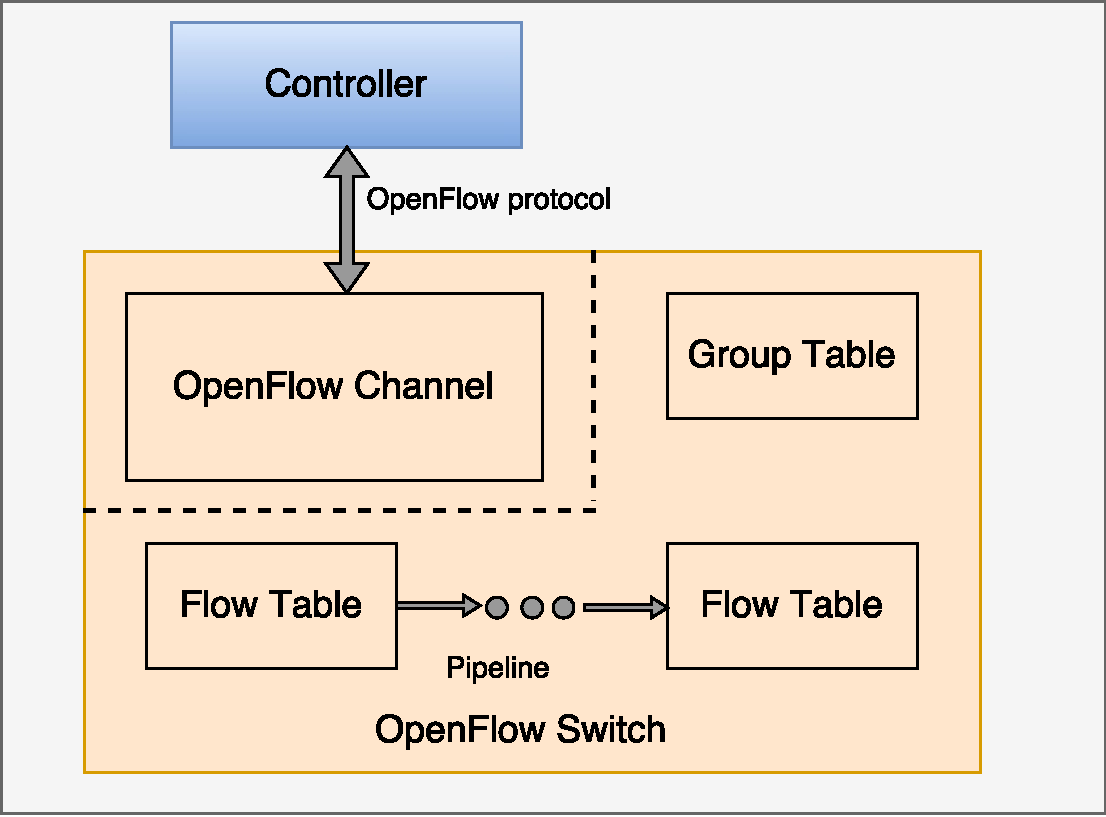
\includegraphics[width=0.75\textwidth]{openflowswitchcomponent.pdf}}
	\caption{Components of an OpenFlow switch \cite{openflowspecification13}.}
	\label{fig:ofscomp}
\end{center}
\end{figure}

\paragraph{Packet Processing}
\paragraph{}
The OpenFlow table entry consists of three fundamental parts, a match field, a counter, and an instruction (see Figure \ref{fig:oftcomp}). The match field dictates what to match in an incoming packet.

\begin{figure}[H]
\begin{center}
	\resizebox{\textwidth}{!}
	{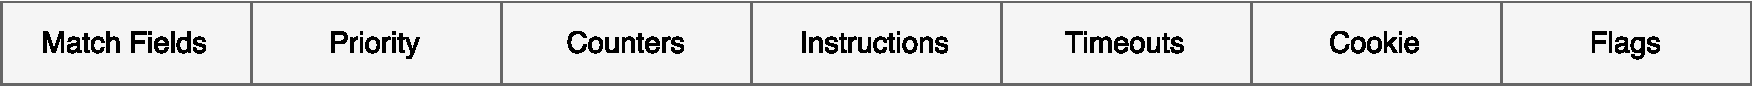
\includegraphics{openflowtablecomponent.pdf}}
	\caption{Components of a flow entry in a flow table \cite{openflowspecification13}.}
	\label{fig:oftcomp}
\end{center}
\end{figure}

On packet arrival, switch matches the header of the packet with the flow entries in a table. If any entry matches, it updates the counters of the entry and performs the specified action. Matching starts at the first flow table and may continue to additional flow tables of the pipeline (see Figure \ref{fig:ofscomp}). The match can happen in a priority order. If no match is found in a flow table for an incoming packet, the outcome depends on the configuration of the table-miss flow entry. For example, the packet may be forwarded to the controller over an OpenFlow channel, dropped, or may continue to the next flow table (see Figure \ref{fig:ofpacketflow}) \cite{openflowspecification13}. Different counters are maintained in OpenFlow, which count the number of packets and bytes at various specific points of the pipeline. There can be a counter for each flow table, flow entry, port, queue, group, group bucket, meter and meter band.

\begin{figure}[H]
\begin{center}
	{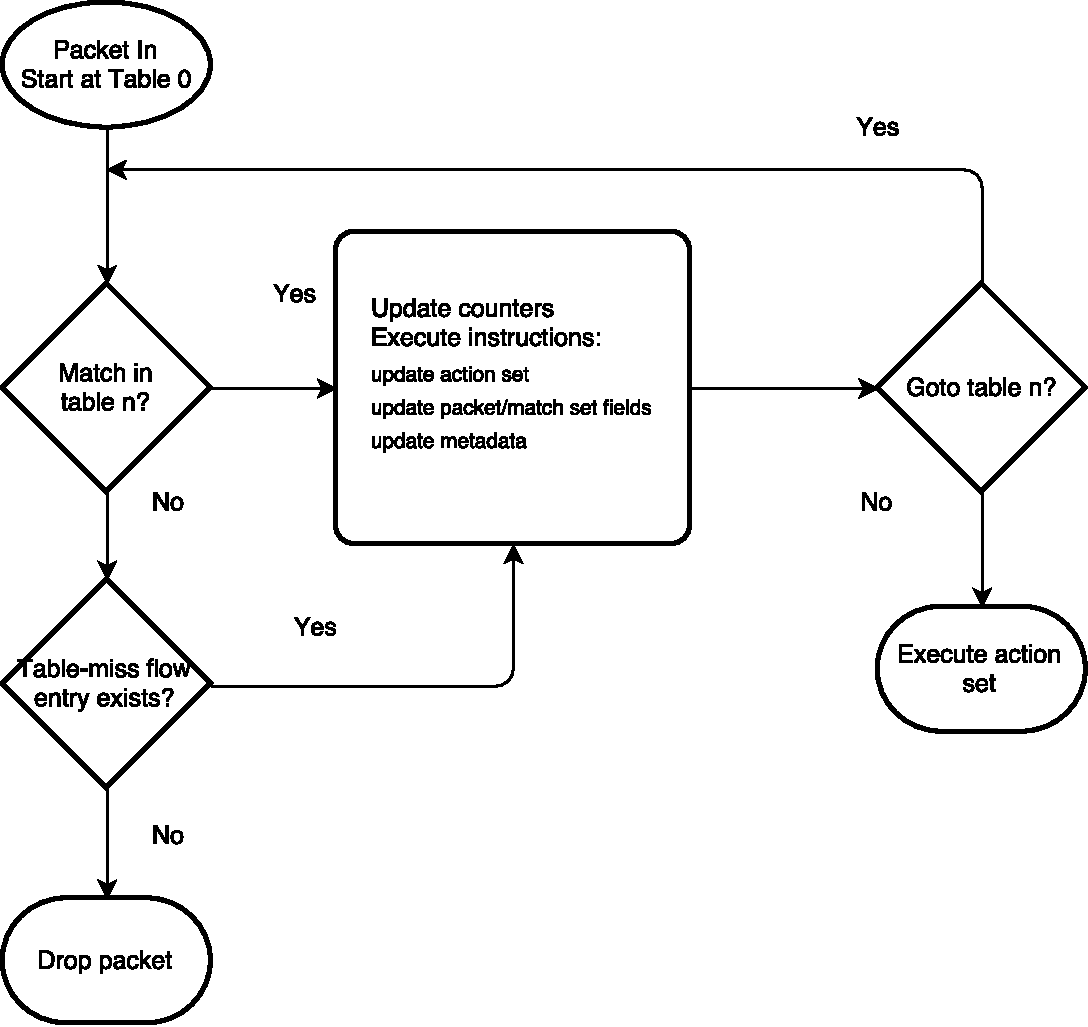
\includegraphics[width=0.75\textwidth]{openflowpacketflowchart.pdf}}
	\caption{Flowchart detailing packet flow through an OpenFlow switch \cite{openflowspecification13}.}
	\label{fig:ofpacketflow}
\end{center}
\end{figure}

Each flow entry consists of an instruction to execute an action on the packet or modify pipeline processing. The valid action could be packet forwarding, packet modification, and group table processing. Pipeline processing passes information in the form of metadata to allow further processing of the packet and sent to the next table. Pipeline processing does not continue when the instruction set associated with a matching flow entry does not mention the next table, which signifies that the packet was already modified and forwarded. Actions associated with flow entries may also direct packets to a group, which means additional processing has to be done. Groups usually represent a set of actions for flooding, as well as more complex forwarding semantics such as multi-path, fast reroute, and link aggregation \cite{openflowspecification13}.

\paragraph{OpenFlow Channel}\label{par:ofc}
\paragraph{}
The OpenFlow channel is the interface that connects each OpenFlow logical switch to an SDN OpenFlow controller; a controller may have connection setup with multiple switches. On the other hand, a switch may have connections with multiple controllers. Having multiple controllers improves reliability as the switch can continue to operate in OpenFlow mode if one controller or the connection fails. Normally, the switch initiates the connection setup with the controller using the host and port configured in the switch. Once the connection channel is set up, communication can happen in both ways, i.e., controller to switch and switch to the controller. The OpenFlow protocol supports three message types: controller-to-switch, asynchronous, and symmetric, each with multiple sub-types \cite{openflowspecification13}. Controller-to-switch messages are initiated by the controller and may or may not require a response from the switch. Asynchronous messages are sent without a controller soliciting them from a switch. Symmetric messages are sent without solicitation, in either direction so any side can initiate a conversation anytime as needed.

\subsection{Open vSwitch}\label{sec:ovs}
Open vSwitch (OVS) is an OpenFlow-capable multi-layer (it can operate at layers 2, 3 and 4) virtual switch. It is typically used with hypervisors to interconnect virtual machines within a host and virtual machines between different hosts across networks. It is also used in some dedicated switching hardware and is an important component in an SDN solution. It works on a number of different platforms including Linux and FreeBSD. It can be configured remotely as well as locally on the box.

\begin{figure}[H]
\begin{center}
	{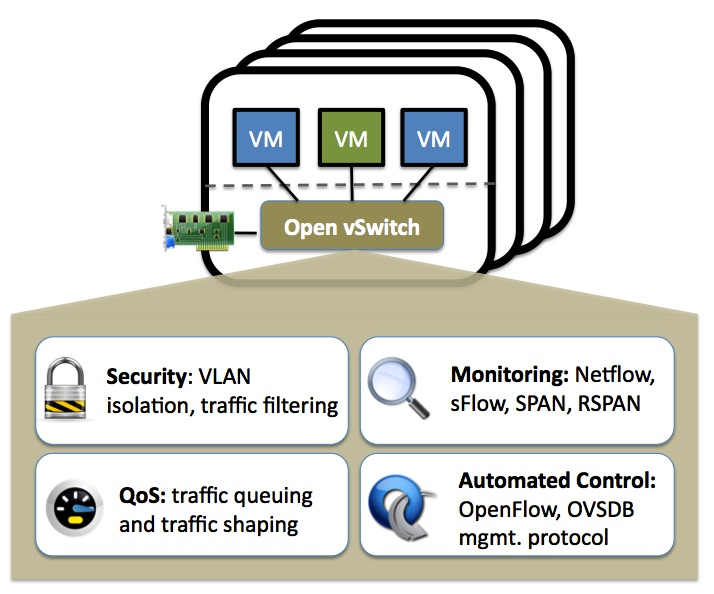
\includegraphics[width=0.75\textwidth]{ovs-overview.png}}
	\caption{Open vSwitch overview \cite{ovswhatis}.}
	\label{fig:ovsoverview}
\end{center}
\end{figure}

Open vSwitch supports many conventional switch features such as Standard 802.1Q virtual LAN (VLAN) model with trunk and access ports, Network interface controller (NIC) port bonding, Link Aggregation Control Protocol (LACP) and various tunnelling method like Geneve, Generic Routing Encapsulation (GRE), Virtual Extensible LAN (VXLAN), Stateless Transport Tunneling (STT), and Locator/ID Separation Protocol (LISP). It also supports many important features like NetFlow, sFlow, mirroring for increased visibility, QoS (Quality of Service) configuration, and policing. It supports OpenFlow 1.0 plus its numerous extensions. OVS can be run in both kernel and user space. It is also included in Linux kernel \cite{ovswhatis}.

\subsubsection{Open vSwitch Components}

\begin{figure}[H]
\begin{center}
	\resizebox{\textwidth}{!}
	{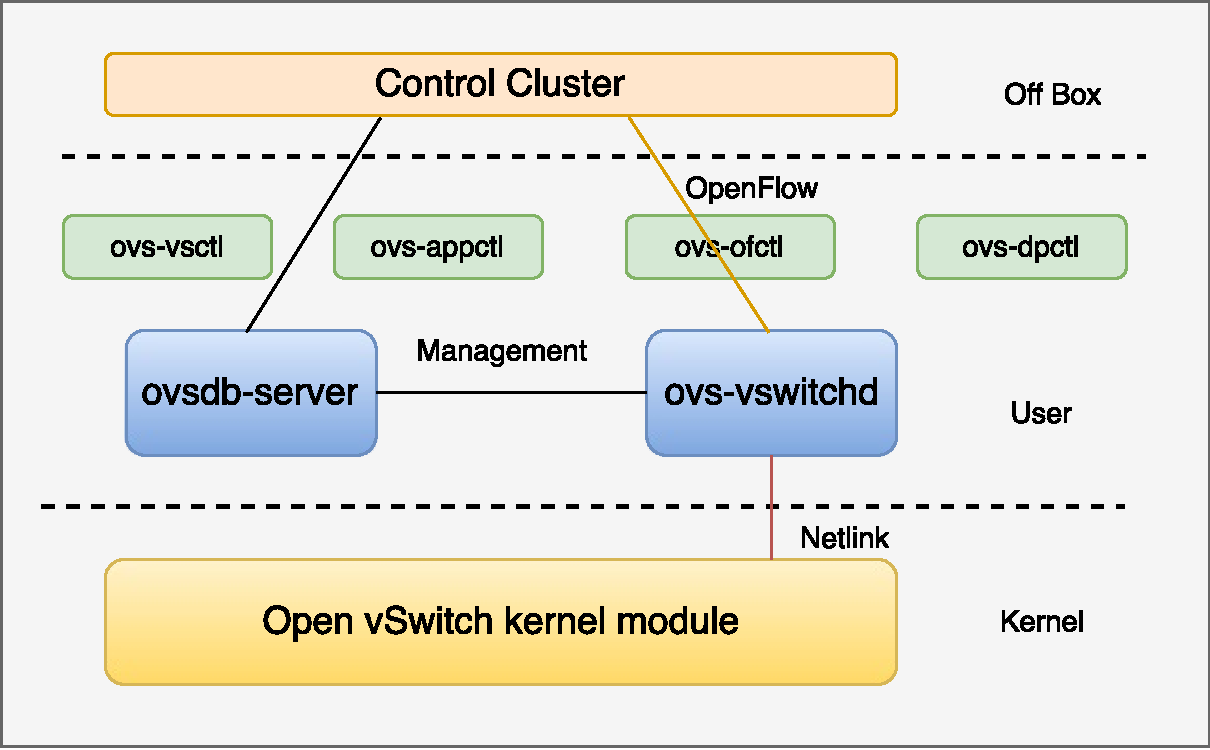
\includegraphics{ovs-components.pdf}}
	\caption{Open vSwitch components.}
	\label{fig:ovscomponent}
\end{center}
\end{figure}

OVS consists of three main components (see Figure \ref{fig:ovscomponent}), ovsdb-server, ovs-vswitchd, and the OVS kernel module. In the upper part of the figure is the control cluster that could be an OpenFlow controller e.g., Ryu, Floodlight, NOX, etc. Ovsdb-server is the component that has the configuration database which is state-full, i.e., information will survive a reboot. It has configuration settings for things like bridges and interfaces. A daemon ovs-vswitchd is the core part of Open vSwitch; it implements the switch and does all of the handlings of flow setups. Open vSwitch kernel module is, in actuality, a cache of recently seen traffic. OVS has different communication protocols (e.g., OpenFlow, Netlink, Management) for improved performance. Different components use them to talk with each other \cite{Pfaff:2015:DIO:2789770.2789779}. The following describes all OVS components in detail:

\paragraph{OVS kernel module:}
The OVS kernel module is mainly responsible for switching and tunnelling and it is a fast cache of non-overlapping flows. It is designed to be fast and simple, it does not know anything about OpenFlow; it simply implements the tunnels.

\paragraph{Ovs-vswitchd:}
Ovs-vswitchd is the core component of the system. It speaks up to the controllers with OpenFlow, to the database server over a management protocol, and it communicates with the kernel module over Netlink on Linux. The command tools that is used to deal with OVS are ovs-vsctl and ovs-appctl.

\paragraph{Ovsdb-server:}
Ovsdb-server holds all the switch level configuration, information about creating bridges, attaches interfaces to bridges, creates tunnels attach to bridges, etc. It also has ovsdb and the OpenFlow controller address. Ovsdb-server stores the configuration eternally and has all the properties of a database. One area of implementation is that it is log-based, i.e., rather than just storing the state of the database, it also contains the changes that have happened, making it very useful for debugging. Ovsdb-server uses a JSON-RPC \cite{jsonrpc}-based protocol for communication.

\paragraph{Ovs-vsctl:}
Ovs-vsctl configures ovs-vswitchd, but it is basically a high-level interface for the database. It can be used for a lot of utilities in OVS, such as configuring the system, looking at the state of the system, among others.

\paragraph{Ovs-ofctl:}
Ovs-ofctl is a utility for querying and controlling OpenFlow switches and controllers. It is used for configuring OVS and uses OpenFlow to the switch, similar to an ovs-vsctl communicating to the ovsdb-server. Typically, ovs-ofctl uses the OpenFlow protocol to the switch over a local socket. Ovs-ofctl can perform operations like dumping the flow table, adding a flow, or deleting flows.

\paragraph{Ovs-dpctl:}
Ovs-dpctl is a tool for configuring the switch kernel module. It can be used to configure the datapath, look at the flow table that has pushed down into the datapath, and dump flows.

\paragraph{Ovs-appctl:}
ovs-appctl is a utility that sends commands to running Open vSwitch daemons. It is used to make changes to or to query the runtime status of the switch.

\section{Flow processing-aware Control Application Placement Framework}\label{sec:fcpf}
Increasing demands of high-quality network service result in different innovative network communication techniques such as CoMP and VNF. These techniques impose more data flow in the network and have several constraints, such as low level of latency and high data rate along with additional processing requirements in the network. Considering all these constraints, accommodating all these techniques requires efficient and flexible management of the underlying backhaul network. 

Recent works \cite{7343600} \cite{aurouxew2017} assume that these techniques can be realized by Control Applications (CAs), acting as functions in the sense of Network Function Virtualization (NFV) \cite{nfv-arch}. Placing these CAs in a suitable location is a challenging task, especially since the traffic load of a mobile network changes very quickly and the performance of a static placement will worsen over time. In modern dense and crowded networks, many data flows appear and expire every second. To reduce reconfiguration overhead, any reassignment should take into account the existing placement. This problem is addressed by a flexible FCAP framework (FlexFCAPF) solution approach. FlexFCAPF places CAs in a suitable location in the network and eventually flexibly reassigns those based on the previous CAs placement in reaction to changes in network load levels.

\begin{figure}[H]
\begin{center}
	\resizebox{\textwidth}{!}
	{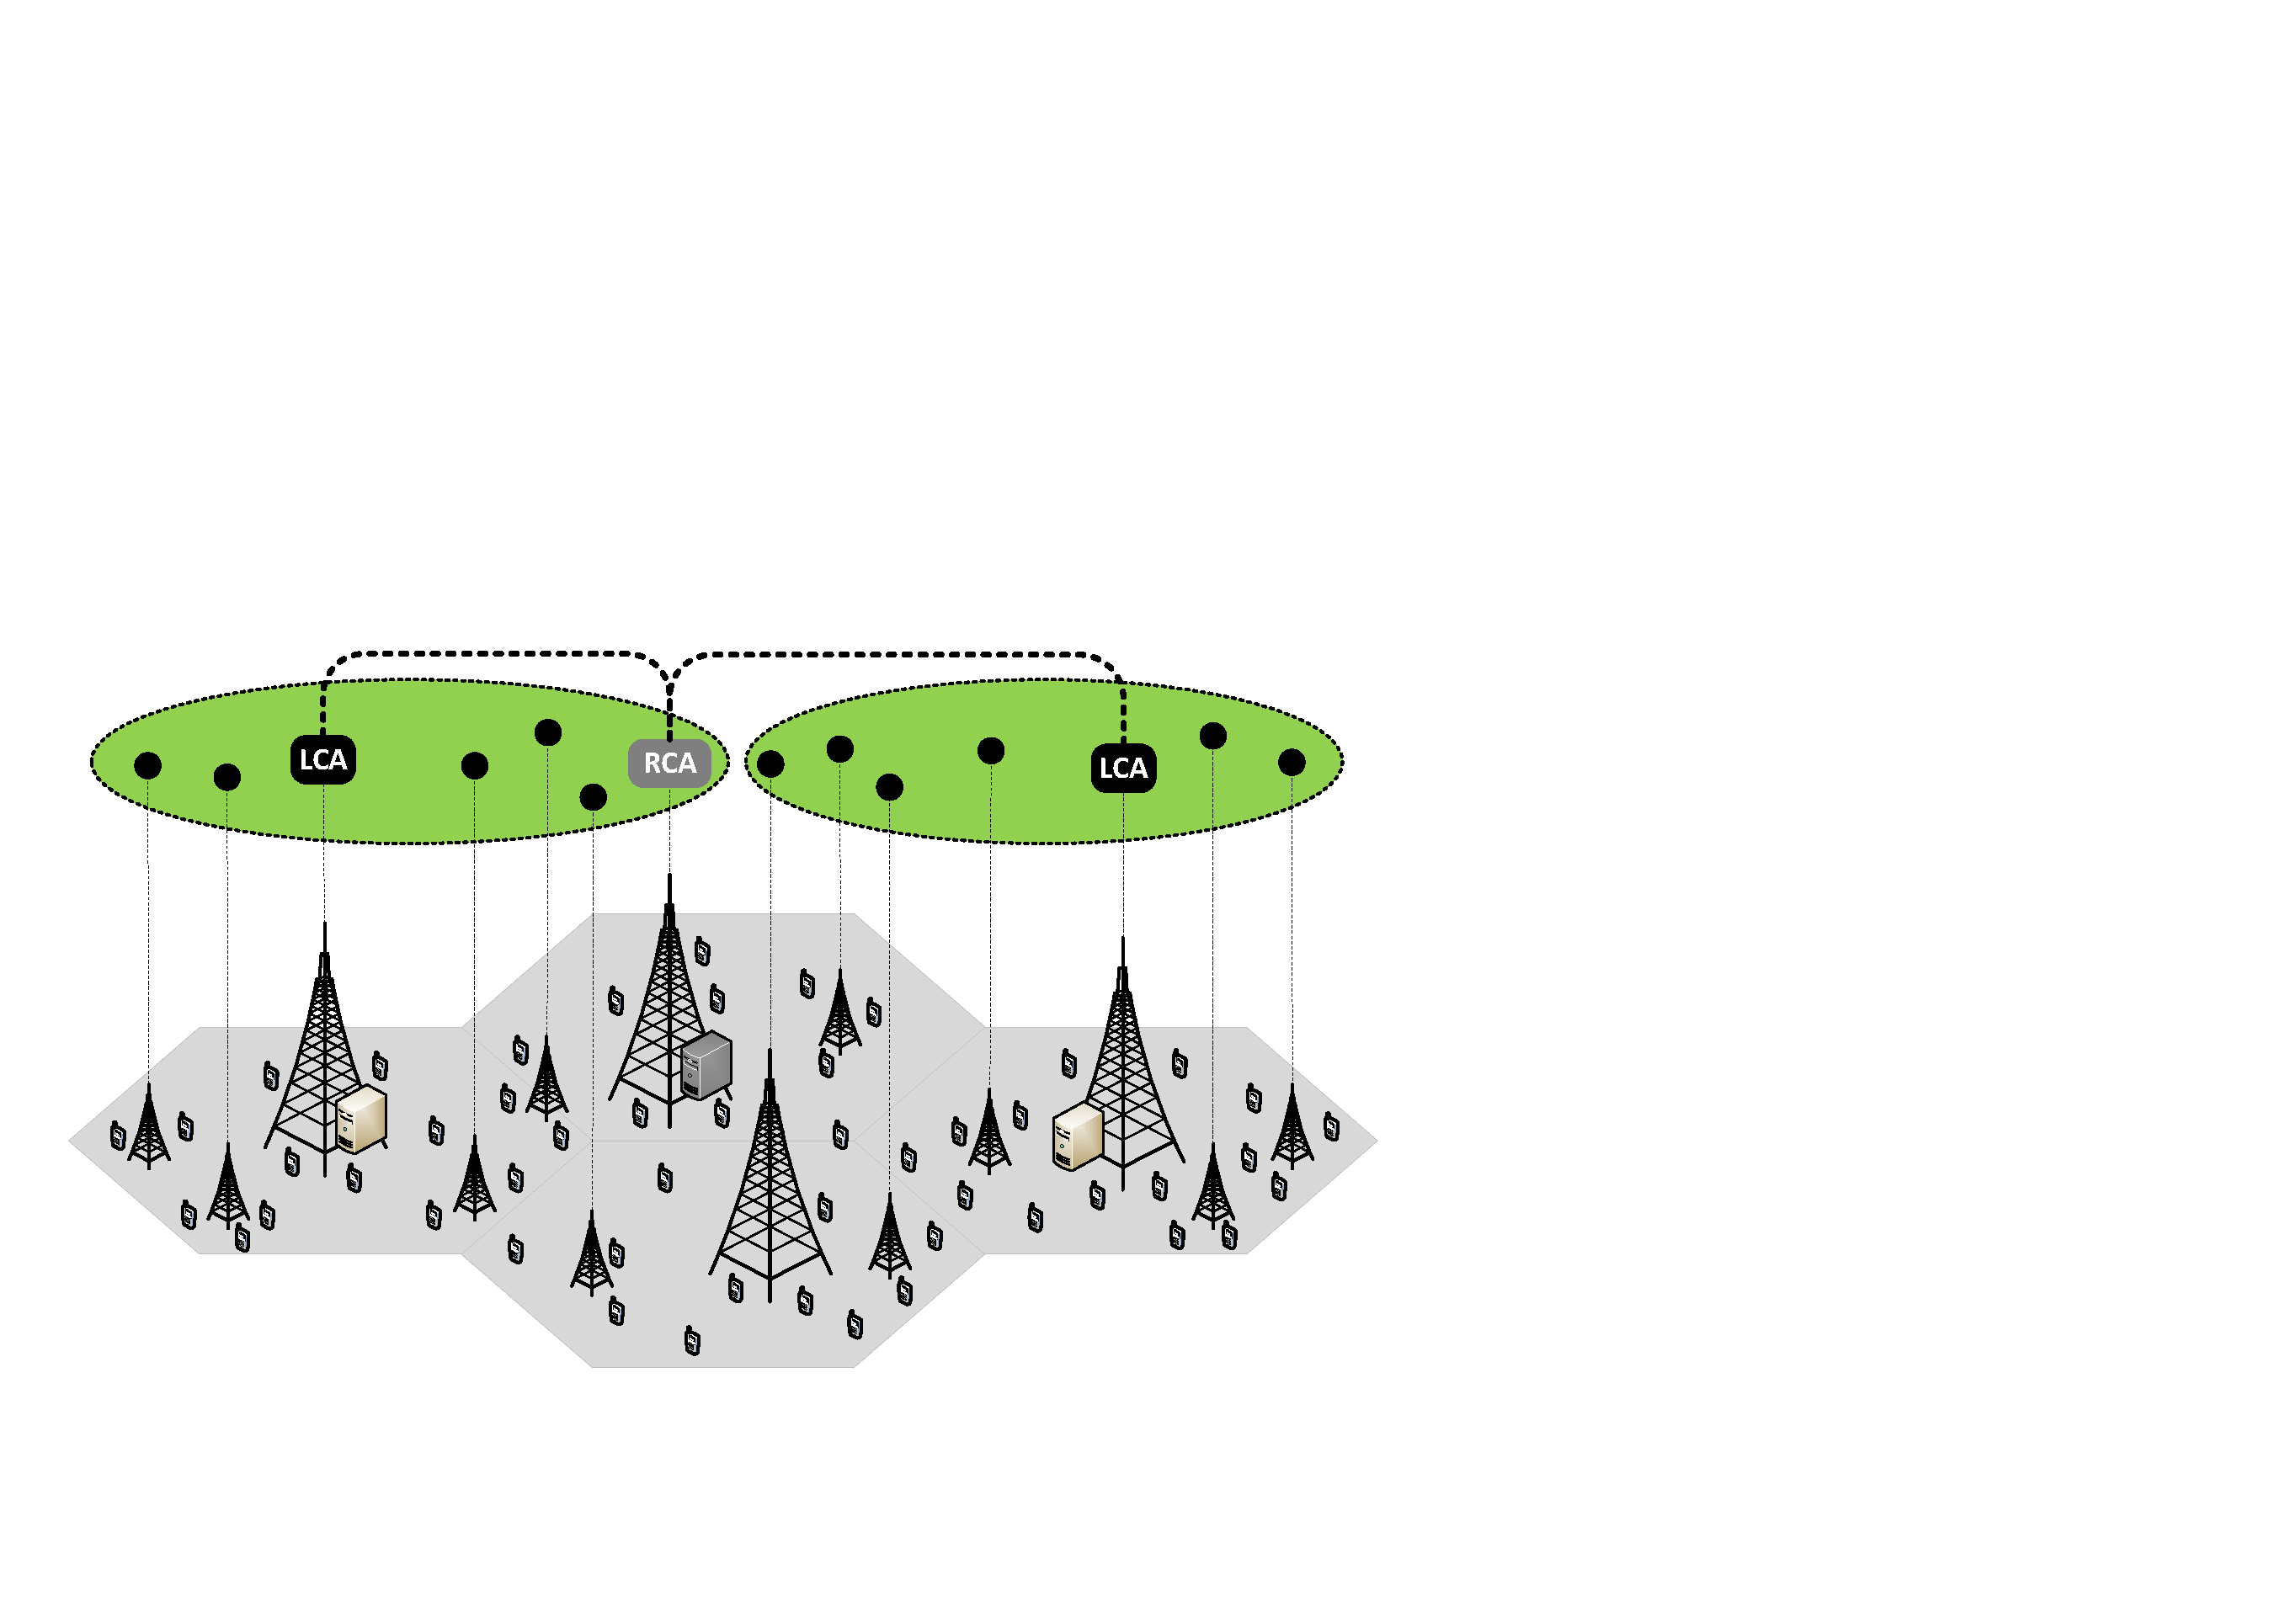
\includegraphics{fcapp-scenario.pdf}}
	\caption{Typical FCAPP framework scenario \cite{aurouxew2017}.}
	\label{fig:fcpfscenario}
\end{center}
\end{figure}

FlexFCAPF architecture consists of a two-tier hierarchical structure of CAs. They are Local Control Applications (LCAs) and Regional Control Applications (RCAs). The LCAs operate locally with limited scope and can execute faster, typically work as a data processing application. The RCAs operate globally with a bigger scope, thus, it can have the myopic view of the local CAs. They typically work as a coordinator of the LCAs. This two-tier hierarchical architecture allows to have a better aggregation of network information, resulting to reduced signaling overhead. Both LCAs and RCAs are seen as CAs acting as functions in the sense of NFV. They can be instantiated on a network equipment that is fulfilling the necessary hardware requirements, i.e., sufficient memory and processing capacity. The high-level coordination of RCAs can be omitted if it is desired. A one-tier hierarchy can be expressed by simply setting all RCA requirements to zero. To illustrate the architecture, Figure \ref{fig:fcpfscenario} shows a typical FlexFCAPF scenario and a possible control structure with one RCA and two LCAs.

FlexFCAPF problem statement and the solution approach are based on the description in \cite{7343600} \cite{aurouxew2017}.
\subsection{FlexFCAPF Problem Statement}\label{sec:ffps}
The job of FlexFCAPF is to place CAs appropriately into a given network, along with satisfying the DFGs available in the network. While doing this, FlexFCAPF considers some constraints such as data processing and latency constraints, along with the network constraints usually associated with network control. FlexFCAPF take an input backhaul network (e.g., Wireless Access Network) as a graph $G = ( V, E )$ with nodes $V$, e.g., switches, and undirected edges $E$, which is representing the links of the network. All nodes in the network may not have the capability of hosting a CA, i.e., fulfill the hardware requirements of becoming a CA, therefore FlexFCPF denotes that capable node by $C \subseteq V$. The processing power of the node is denoted by $p_{node} ( c )$ FLOPS where $c \in C$. The link between two node is denoted by $( u, v ) \in E$ and a link has a maximum data rate of $b_{cap} ( u, v )$ bit/s and a latency of $l_{cap} ( u , v )$ seconds. FlexFCAPF considers the latency of a link independent of the network load and ignores possible queuing delays.

A solution of the given network is achieved by creating a complete control structure, i.e., each node of the network $v \in V$ is controlled by at least one LCA (a node can be controlled by more than one LCA if needed for optimal network performance) and each LCA is required to be coordinated by exactly one RCA. An LCA needs a processing capacity of $p_{LCA}$ FLOPS per controlled node for becoming the LCA of a node while an RCA needs a processing capacity $p_{RCA}$FLOPS per coordinated LCA for becoming the RCA of an LCA. Also, a path must exist between a node and its LCA and a round trip latency cannot be more than $l_{LCA}$ seconds and should provide a minimum data rate of $b_{LCA}$ bit/s. The routing path between a node and its LCA needs to have at most a round trip latency of $l_{LCA}$ seconds and a minimum data rate of $b_{LCA}$ bit/s. Similarly, the path between an LCA to its RCA need to have a round trip latency $l_{RCA}$ seconds and a minimum data rate of $b_{RCA}$ bit/s.

Furthermore, FlexFCAPF denotes the Data Flow Groups (DFGs) on the network as a set $F$. Each DFG contains one or multiple (to represent scenarios like CoMP) data flows, and enters the backhaul network through a node from $V$. The data flows of one DFG may originate from different nodes in the network but all of them has to be processed by the same LCA jointly. The connection matrix $W \in \{ 0, 1 \}^{| F | \times | C |}$ is used to represent the relationship between DFG and the set of network nodes. The processing LCA of a DFG should provide a processing power of $p_{flow} ( x )$ FLOPS for processing every data flow from each DFG $x \in F$. The routing path between the LCA and the nodes through which the DFG is entered in the network need to provide a maximum round trip latency $l_{flow} ( x )$ seconds and a data rate of $b_{flow} ( x )$ bit/s. For simplicity, FlexFCAPF considers the full round trip for all DFGs, so that FlexFCAPF solution fully incorporates request and response traffic.

A DFG $x \in F$ is said to be satisfied by an LCA $c \in C$ if and only if
\begin{enumerate}
	\item $c$ controls all nodes $v$ with $W_{x,v} = 1$ and
	\item the routing paths from all nodes $v$ with $W_{x,v} = 1$ to $c$ have sufficient resources to provide a data rate of $b_{flow} ( x )$ and a round trip latency $l_{flow} ( x )$.
\end{enumerate}

It is important to remember, that the round trip latency in the network is not only the travel time of the data flow. It also includes the time necessary for processing the data flow $x$ at $c$. Therefore, to enable a round trip latency $l_{flow} ( x )$, a sufficient amount of processing capacity from $c$ has to be allocated for $x$ to handle $p_{flow} ( x )$ FLOPS and the link delays in time.

\subsection{FlexFCAPF Solution Approach}
The objectives of FlexFCAPF are as follows, listed in descending order of importance:
\begin{enumerate}
	\item Create a valid solution, i.e. a complete control structure,
	\item Maximize the number of satisfied DFGs, and
	\item Minimize the number of used CAs.
\end{enumerate}

The main objective of FlexFCAPF model is to provide a fully functional valid network solution, i.e., a complete control structure with the maximum number of DFGs are satisfied by an LCA. However, DFGs being satisfied at any point of time may not be possible at all events. This is because the network might have many DFGs entered at some point in time but it does not have enough resources to satisfy all. In such a situation, FlexFCAPF might result in an incomplete control structure, i.e., not all nodes are correctly controlled, which is why creating a complete control structure is more important for the network than a couple of yet unprocessed DFGs. Saving network resource is an important objective from an operator's point of view and minimizing the number of used CAs is preferred in saving such costs. On the other hand, dropping DFGs would reduce Quality of Service (QoS) and will eventually frustrate customers. Therefore, minimizing the number of used CAs is given less importance than DFG satisfaction and feasible only if it does not affect the network's performance.

My considered version of FCAPP assumes that the schedule for data processing at an LCA is First Come First Serve (FCFS) scheduling. This means that the LCA will allocate the requested processing power by any DFG and that particular DFG will hold that amount of processing power until it finishes the job. The LCA will also allocate the amount of processing power required by all its controlled nodes. FlexFCAPF determines the required routing paths to guarantee that no constraint for network control and DFG processing is violated, and verifies that all conditions are satisfied at any point in time. The implementation of the algorithm will be elaborated in section \ref{sec:algoadap}.

\section{Tools and Technology}\label{sec:tools}
The different approaches of testing computer network application was described in section \ref{sec:nta}. Simulation and emulation provide a solid base to determine the pros and cons of a netwrok application. However, emulation is more realistic than simulation since it must be carried out in real time and could provide a way to some real devices running real operating systems to interact with some simulated devices \cite{6588659}. Moreover, recent works \cite{7343600} already evaluated FlexFCAPF model by simulation. In this study, FlexFCAPF will be evaluated in the emulation environment, thus selecting appropriate tools and technologies for building an emulation testbed is necessary. The following paragraph describes the basis for selecting those tools and technologies. A brief description of their features and functionalities is also given in the later section.

First, a platform had to be chosen where FlexFCAPF can be adapted easily. There are not many SDN platforms available for use, and for these Mininet \cite{Lantz:2010:NLR:1868447.1868466}, MaxiNet \cite{6857078}, EstiNet \cite{6588659}, NS-3 \cite{ns-3}, DOT \cite{6838241} and OFnet \cite{ofnet} were compared. NS-3 is an open source platform and available free of use. It has an OpenFlow simulation model and it offers a realistic OpenFlow environment. However, it does not support real OpenFlow controllers, so they developed their own controller but it does not support latest OpenFlow protocol \cite{al2014survey}. 

EstiNet is one of the best emulators which provide correct, trustworthy performance result and high scalability \cite{6588659}. EstiNet provides distributed emulation across multiple machines with an added feature of time dilation. However, there are not many details available about the technique used by EstiNet and how to use it as it is a closed-source proprietary platform. 

DOT is a low cost and scalable network emulator. In the paper \cite{6838241}, DOT is claimed to emulate large-scale SDN deployment, overcoming the scalable limitation of Mininet. The paper also suggested that DOT provides guaranteed CPU time, bandwidth, and network latency for the emulated components (i.e., switches, hosts, and links). It scales with the network size and traffic volume, has a built-in central system for configuring and monitoring the emulated components, and makes it possible to run any customizable controller. DOT looks like a promising option for the testbed setup since it matches most of my testbed requirements, except for data processing capability. It was not specified, however, how scalable the environment is and no practical example to use DOT was given, neither any reliable implementation example can be found. 

OFnet is another easy-to-use platform to setup SDN network emulation and it comes with a friendly Apache v2 license. It provides some interesting features such as visual debugging of control plane transactions and traffic generation on emulated network. Developers claim these features enable the user in characterizing the performance of an SDN controller. The traffic generation feature of OFnet is interesting for my testbed but it does not provide much flexibility such as in generating controlled traffic. Similar to DOT, OFnet also lacks practical implementation and is not usually used in testing. 

Mininet is one of the most popular SDN platform used by many SDN researchers because of its simplicity, availability, and flexibility. It also fully supports OpenFlow architecture \cite{Lantz:2010:NLR:1868447.1868466}. However, Mininet is not scalable and can not be deployed over multiple machines. This limitation is resolved in MaxiNet. MaxiNet is basically an extended platform based on Mininet which can be deployed over multiple servers connected via a network. Since MaxiNet supports the existing Mininet API with minimal alteration and Mininet has been used in many SDN testbed emulations projects, I decided to use Mininet for small-scale testing and MaxiNet for large-scale testing.

One important aspect of FlexFCAPF model is that it generates the flow path of the traffic flow it satisfies as part of the solution. Therefore, an OpenFlow controller is needed which can be used to configure the generated flow path in the network dynamically. The OpenFlow controller should be easily customizable, compatible to Mininet/MaxiNet, component-based. For this purpose, NOX \cite{nox}, POX\cite{pox}, Floodlight \cite{floodlight}, OpenDaylight \cite{opendaylight} and Ryu \cite{ryu} were compared. 

NOX controller is one of the first controllers of OpenFlow written in C++ language. Its first version provides an API for Python scripts, but the last version of NOX has dropped the API support and kept only C++. NOX provides a high-level, programmable interface upon forwarding devices and applications. It is designed to support both small networks of a few hosts and large enterprise networks of hundreds of switches and hosts. NOX's core has features of fast, asynchronous I/O, topology discovery, host tracking possibility, and learning switch feature. Researchers discovered that NOX does not support the iperf command properly which determines the bandwidth utilization \cite{al2014survey} and is an important requirement for this study's testbed since iperf will be used to generate controlled traffic. NOX's documentation support is very poor and its mailing-lists are almost abandoned. 

POX is the younger sibling of NOX; the main difference is that it is developed in Python instead of C++. POX uses Python API to support network virtualization, SDN debugging, and different applications such as layer-2 switch, bridge, hub, among others \cite{al2014survey}. Again, its documentation support is very poor. 

Both Floodlight and OpenDaylight are very popular SDN controllers and developed in Java-based platform, thus it runs within a Java Virtual Machine (JVM). Compared to Floodlight, OpenDayLight is more modular, extensible and scalable, but it has an issue with iperf command similar to NOX \cite{al2014survey}. 

Ryu is a component-based, open source framework implemented entirely in Python. Ryu messaging service also supports components developed in other languages \cite{ryu}. Ryu controller includes application management, in-memory state management, event management, and series of reusable libraries (e.g., NetCONF library, sFlow/NetFlow library, and OF-Config library). Ryu supports services like topology discovery, asynchronous I/O, and learning switch feature which are very useful. Ryu is well documented and it has an active mail support group. In \cite{6916572}, a detailed analysis based on multiple parameters (Interface, Platform supports, REST API, Productivity, Documentation, Modularity) was executed and Ryu was selected as the best controller based on the cumulative weighting. Therefore, I selected Ryu framework for developing a custom SDN controller for the testbed.

In the following section, features and functionalities of the selected tools and technology used in this study are written in detail.

\subsection{Mininet}\label{sec:mininet}
Mininet is a network emulation software that allows creation of a realistic virtual network with real networking component by executing a single command on a single machine (VM, cloud, or native). Mininet hosts are implemented to run standard Linux network software and its switches (e.g., Open vSwitch or Linux Bridge) support OpenFlow for highly flexible custom routing and SDN. Mininet can be used for the various purpose of research, development, learning, prototyping, testing of SDN applications, and OpenFlow. Emulation using Mininet runs a real code and it supports running standard Linux network applications including network stack and the real Linux kernel. Because of this, a newly developed OpenFlow controller, modified switch, or host, can be moved to a real system with little changes, for real-world testing, performance evaluation, and deployment. Using Mininet is an effective way to test network for different system behavior and experiment with topologies \cite{min-over}.

\subsubsection{Mininet Components}

\begin{figure}[H]
\begin{center}
	\resizebox{\textwidth}{!}
	{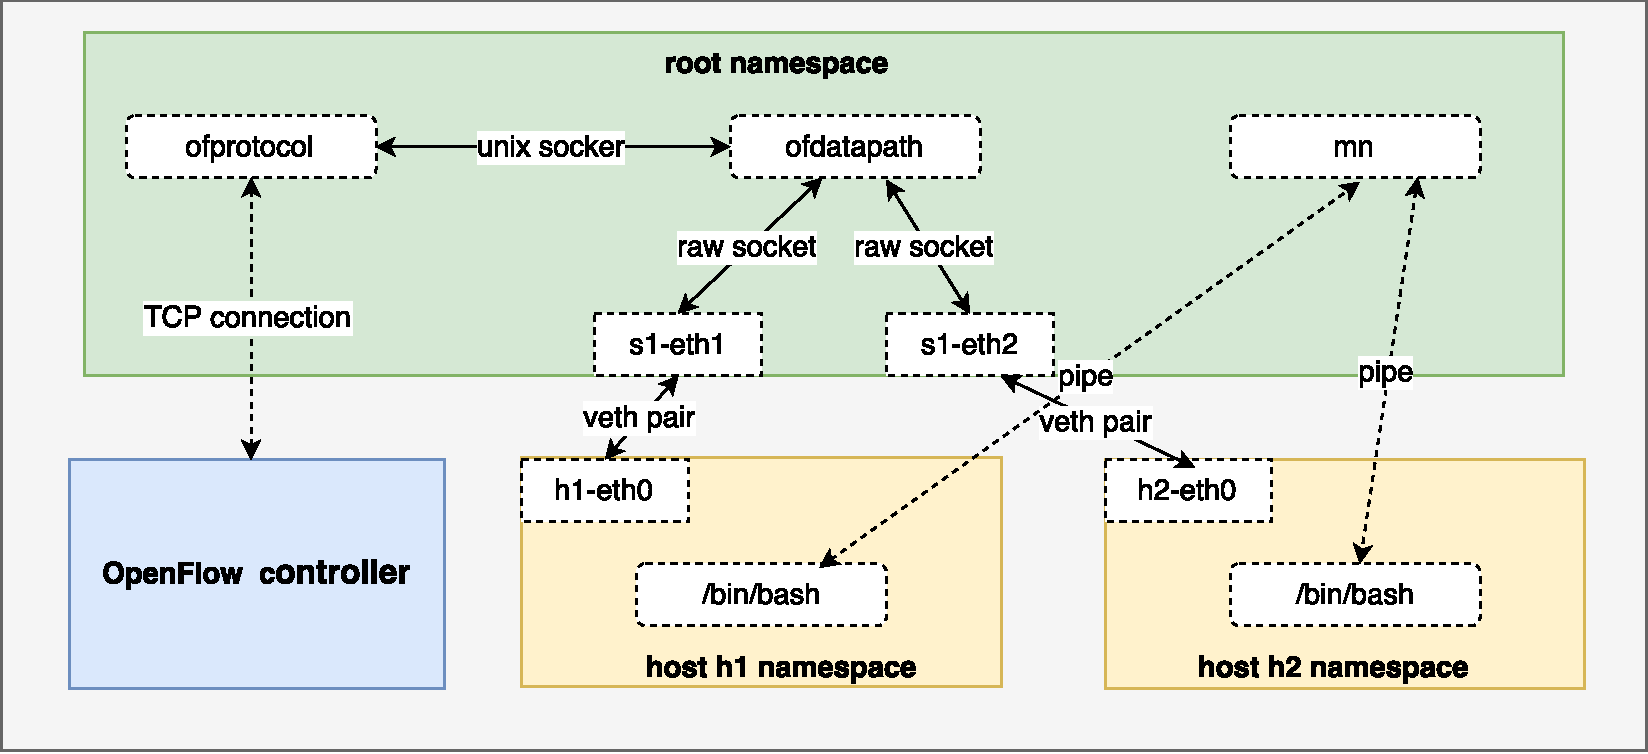
\includegraphics{mininet-components.pdf}}
	\caption{Mininet components \cite{Lantz:2010:NLR:1868447.1868466}.}
	\label{fig:mincomponent}
\end{center}
\end{figure}

Mininet uses the built-in Linux OS kernel's lightweight virtualization mechanism. It uses different useful Linux features like network namespaces, process groups, and CPU bandwidth isolation and combines them with virtual Ethernet links and link schedulers. These in-build features of Linux helps Mininet to start faster and also gives flexibility to scale the system with hundreds of hosts and switches on a single machine. This is not possible in emulators which use full virtual machines \cite{Lantz:2010:NLR:1868447.1868466}. A Mininet network consists the following components (see Figure \ref{fig:mincomponent}):

\paragraph{Network Namespace:}
Network namespaces are the container \cite{container} for network state. It provides processes (or group of processes) with exclusive ownership of interfaces, ports, and routing tables (such as ARP and IP). With network namespace, one can have different and separate instances of network interfaces and routing tables that operate independently of each other \cite{Handigol:2012:RNE:2413176.2413206}.

\paragraph{Hosts:}
A Mininet host is basically a shell process (e.g., bash) moved into its own network namespace with the unshare (CLONE NEWNET) system call. Each Mininet host has its own virtual Ethernet interface(s) and a pipe to a parent Mininet process (i.e., mn)(see Figure \ref{fig:mincomponent}), which sends commands and monitors output. Mininet uses Linux functionality of hierarchical scheduling, resource management, and CPU Bandwidth limiting features to limit the fraction of a CPU available to each process group \cite{cgroups-man} \cite{Handigol:2012:RNE:2413176.2413206}.

\paragraph{Links:}
A Mininet Link is basically a virtual Ethernet pair or veth pair\cite{container}. It acts like a wire connecting between two virtual interfaces. Each interface acts like a fully functional ethernet port to all systems and application software. Packets sent through one interface are delivered to the other interface of the veth pair. A veth pair may be attached to virtual switches such as the Linux bridge or an OpenFlow software switch. The data rate of each link can be configured, which is achieved by using Linux Traffic Control (\textit{tc}) \cite{tc-man}, which has a number of packet schedulers to shape traffic to a configured rate \cite{Handigol:2012:RNE:2413176.2413206}.

\paragraph{Switches:}
Mininet typically uses the default Linux bridge or Open vSwitch running in kernel mode to switch packets between interfaces. These software OpenFlow switches provide similar packet delivery facilities that would be provided by a hardware switch. Both user-space and kernel-space switches are available. Usually switch runs in the kernel for better speed \cite{Handigol:2012:RNE:2413176.2413206}.

\paragraph{Controllers:}
Mininet Controllers can be an external or internal process running anywhere on the real or simulated network. The controller should provide IP-level connectivity to the machine on which the Mininet switches are running. For example, for Mininet running in a VM, the controller could run inside the VM, natively on the host machine, or in the cloud \cite{Handigol:2012:RNE:2413176.2413206}.

\subsubsection{Mininet Advantages}
Mininet combines many of the best features of simulators, emulators, and real network testbeds \cite{min-over}.
\begin{itemize}
	\item Starting up a simple Mininet network takes just a few seconds.
	\item Mininet allows creating custom topologies, e.g., a data center network, large Internet-like topologies, or a simple single switch network.
	\item It is possible to run any real programs (e.g., a web server, TCP monitoring tool, or Wireshark) that can be run on Linux.
	\item It is simple to create and run Mininet experiments by writing simple (or complex) Python scripts.
	\item Mininet's switches are programmable using the OpenFlow protocol, so one can easily develop a custom SDN controller and implement customized packet forwarding logic as necessary.
	\item Mininet can be run on a laptop, on a server, or in a VM.
	\item Mininet provides a straightforward and extensible Python API for network creation and experiments.
	\item Mininet has a Command Line Interface (CLI) that is topology-aware and OpenFlow-aware; thus, very useful for debugging or running network-wide tests.
	\item Mininet provides a simple and inexpensive network testbed for developing and testing OpenFlow network applications.
	\item There is an active community mail-group for discussion about various features and problem about Mininet.
\end{itemize}


\subsubsection{Mininet Limitations}
Mininet is a great tool for networking experiments, but it does have some limitations as well \cite{min-intro}.
\begin{itemize}
	\item Mininet has a resource limitation concern. Mininet-based networks currently cannot exceed the CPU or bandwidth available on a single machine. This problem can be resolved in MaxiNet, which is described in section \ref{maxinet}.
	\item Mininet, currently, cannot run non-Linux compatible OpenFlow switches or applications. Software that depends on BSD, Windows, or other operating system kernels can not be run on Mininet.
	\item All Mininet hosts share the host file system and PID space. The user has to be careful with the daemon process running on Mininet host, if they require configuration in /etc or in shared common place.
	\item It is not easy to use virtual time in Mininet to achieve faster than real-time results, such as in simulation.
	\item One has to write own OpenFlow controller if custom routing or switching behavior is needed in the network. It is, however, easy to combine any OpenFlow controller to run with Mininet network.
\end{itemize}

\subsection{MaxiNet}\label{maxinet}
MaxiNet is a highly scalable, distributed emulation environment for large SDNs \cite{max-over}. MaxiNet is basically an extension of the Mininet emulation environment. Mininet has a drawback of not being able to run across multiple physical machines and for this reason, Mininet is not highly scalable. MaxiNet resolves these problems by distributing nodes between multiple physical hosts. MaxiNet achieves the distributed functionality by running on a cluster of several physical machines (called \textit{Worker}) connected by a physical network. Through this, MaxiNet distributes a part of the whole network between these workers and each of these workers runs a Mininet emulation on it. MaxiNet uses Generic Routing Encapsulation (GRE) tunnels to interconnect switches and hosts spread across different workers. The workers communicate through the physical network to pass traffic across the workers. By using MaxiNet, a large virtual network of thousands hosts and switches can be emulated with multiple numbers of workers. MaxiNet coordinates between these isolated Mininet emulation using a centralized API invoked in a specially-designed worker called \textit{Frontend}. The main job of the frontend is to partition the whole network into smaller units and distribute these smaller networks into the workers. Frontend also keeps track of which node resides on which worker. This way, one can easily access all nodes through the frontend. The frontend can also be configured to act as a worker and it has to be done manually before starting the experiment. Through this, MaxiNet allows emulating very large SDN testbed in a very convenient way \cite{6857078}.

\begin{figure}[tb]
\begin{center}
	\resizebox{\textwidth}{!}
	{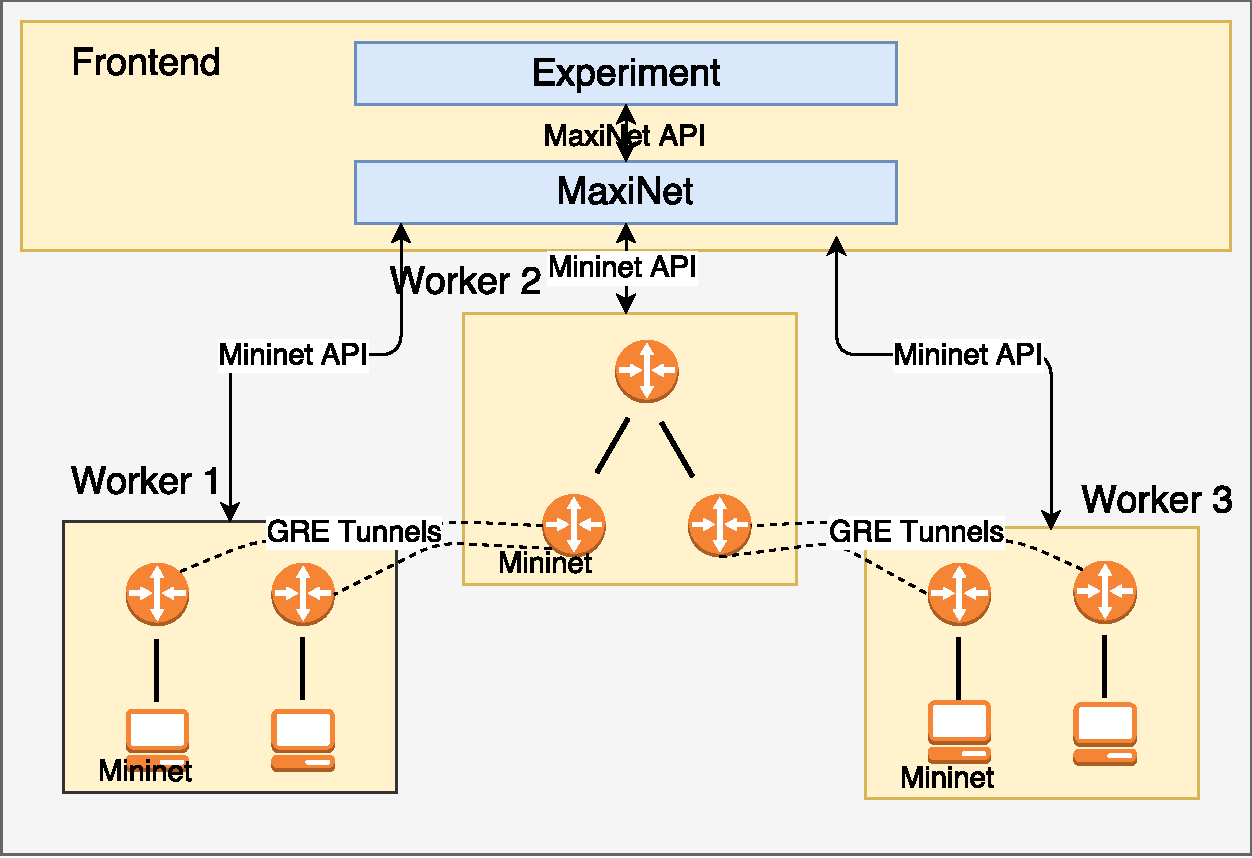
\includegraphics{maxinet-overview.pdf}}
	\caption{Schematic view of MaxiNet \cite{6857078}.}
	\label{fig:maxoverview}
\end{center}
\end{figure}

Figure \ref{fig:maxoverview} shows the schematic view of MaxiNet. A user provides a topology to the MaxiNet Experiment in the frontend to set up a network. The Experiment uses MaxiNet API to pass that information to MaxiNet. MaxiNet partition that topology into several smaller virtual network to distribute among the workers. MaxiNet uses the graph partitioning library METIS \cite{Karypis95metis--} for partitioning. METIS computes the partitions, dividing the total nodes almost equally among the workers. The aim of the partitioning process is to restrain most of the emulated traffic locally to the workers. Each MaxiNet worker takes these divided units assigned to them and instantiate a Mininet network in their system. MaxiNet uses Mininet API to control the workers and uses RPC calls to communicate with them. The worker uses GRE tunnels to communicate among the nodes between them. MaxiNet API can be used to set up, control, and shut down a virtual network and it is designed similarly to Mininet API to ease the use of MaxiNet among Mininet users \cite{6857078}.
 
\subsubsection{MaxiNet Advantages and Limitations}
Since MaxiNet is a distributed enhancement of Mininet it has similar advantages and disadvantages to Mininet. One major advantage of MaxiNet is it can be scalable up to thousands of nodes (switches and hosts) and can be distributed among multiple physical machines. However, as a disadvantage, its CLI support is not vast; it would have been helpful to have all Mininet command supported in MaxiNet. The data rate between nodes on different workers is very less compared to the nodes on same worker. Its documentation is poor but not a major drawback as there are many support groups available for Mininet.

\subsection{Ryu SDN Framework}\label{sec:ryu}
Ryu is a component-based open source platform for building SDN applications. Ryu is designed based on the philosophy of agility and flexibility in mind; thus, it is easy to manage. Ryu supports various protocols for managing network devices, such as OpenFlow (1.0, 1.1, 1.3, 1.4, 1.5), NetCONF, and OF-config, among others. Ryu provides software components with well-defined APIs. It is easy for developers to create new network management and controller applications using Ryu. One can easily modify an existing component and build a new component or implement his own component. It is easy to combine multiple Ryu components and build a Ryu application based on the specific requirements of a developer to ensure that the underlying network can meet the demands. A component of Ryu is basically separation functional unit and they communicate by passing messages instead of directly referencing each other. Existing components of Ryu are implemented in Python and a component consists of python thread or OS process \cite{ryu}. Figure \ref{fig:ryufwis} shows how Ryu framework fits in the SDN.

\begin{figure}[tb]
\begin{center}
	\resizebox{\textwidth}{!}
	{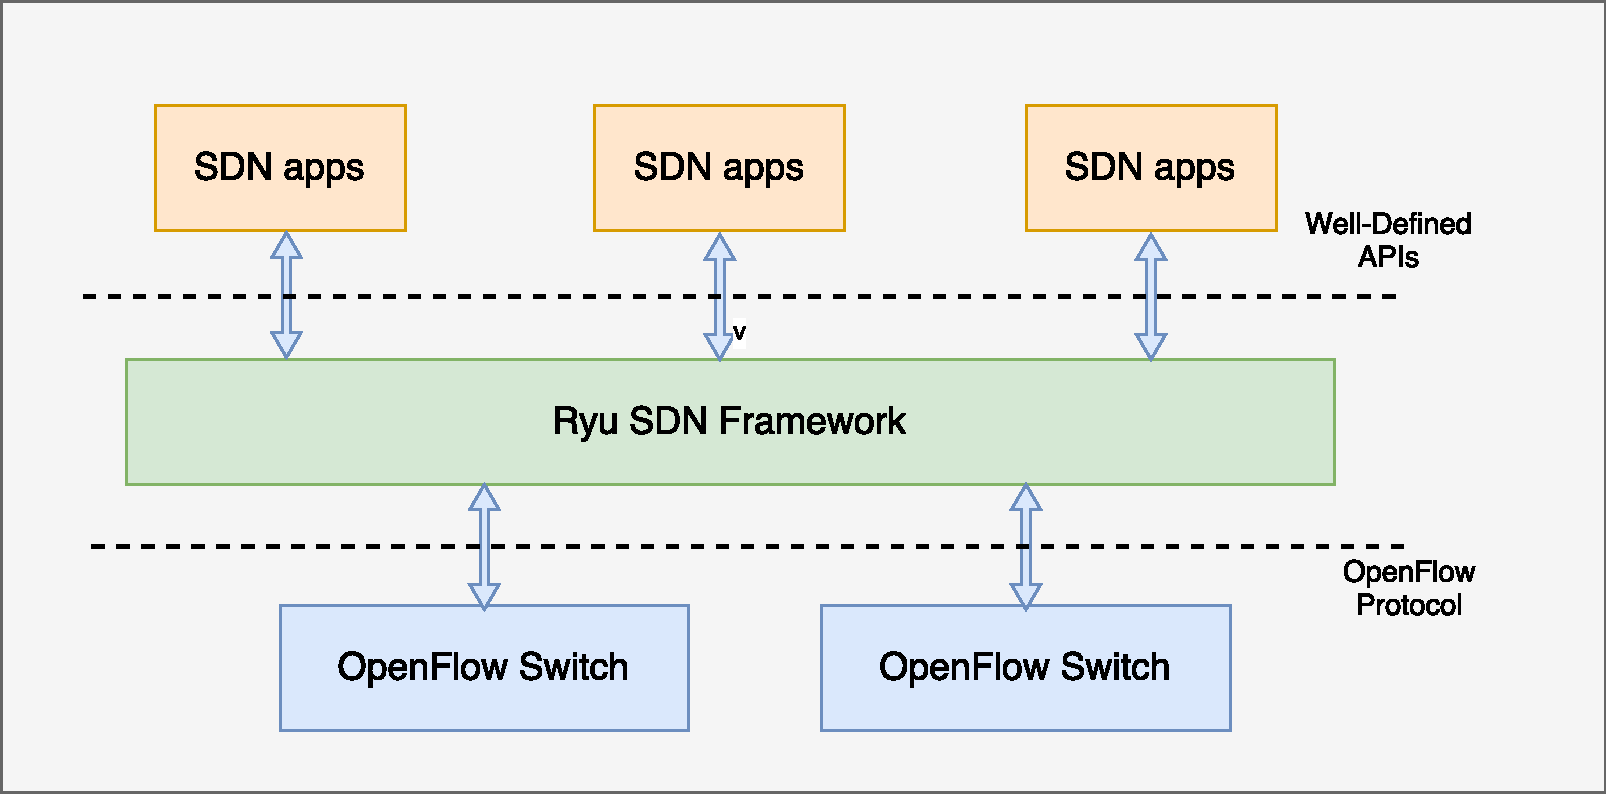
\includegraphics{ryu-frameworkinsdn.pdf}}
	\caption{Ryu framework in SDN.}
	\label{fig:ryufwis}
\end{center}
\end{figure}

As part of this study, a controller application is developed using some of the components of Ryu SDN framework. It uses OpenFlow 1.3 to interact with the forwarding plane (switches and routers) to modify how the network will handle traffic flows. Some Ryu component descriptions used in the SDN controller of the testbed are listed below.

\paragraph{ryu.base.app\_manager:}
This is the central management of a Ryu application. It is responsible for loading the application, providing context to the application, and routing messages between Ryu applications.
\paragraph{ryu.controller.controller:}
This is the main component of an OpenFlow controller. It handles connections from the switches and generate events and route them to appropriate entities like Ryu applications.
\paragraph{ryu.controller.dpset:}
This manages switches.
\paragraph{ryu.controller.ofp\_event:}
This is the class for OpenFlow event definitions.
\paragraph{ryu.controller.ofp\_handler:}
This is the handler of basic OpenFlow handling including negotiation.
\paragraph{ryu.ofproto.ofproto\_v1\_3:}
This is the class for OpenFlow 1.3 definitions.
\paragraph{ryu.ofproto.ofproto\_v1\_3\_parser:}
This module implements OpenFlow 1.3.x.
\paragraph{ryu.topology:}
This is the Switch and link discovery module.

\subsubsection{Ryu Application Programming Model}
This section explains the Ryu application programming model (see Figure \ref{fig:ryuarch}). To understand the SDN Controller (see Section \ref{sec:fca}) flow developed for this study, it is important to know the Ryu application programming model \cite{ryuapm}.

\begin{figure}[H]
	\begin{center}
		\resizebox{\textwidth}{!}
		{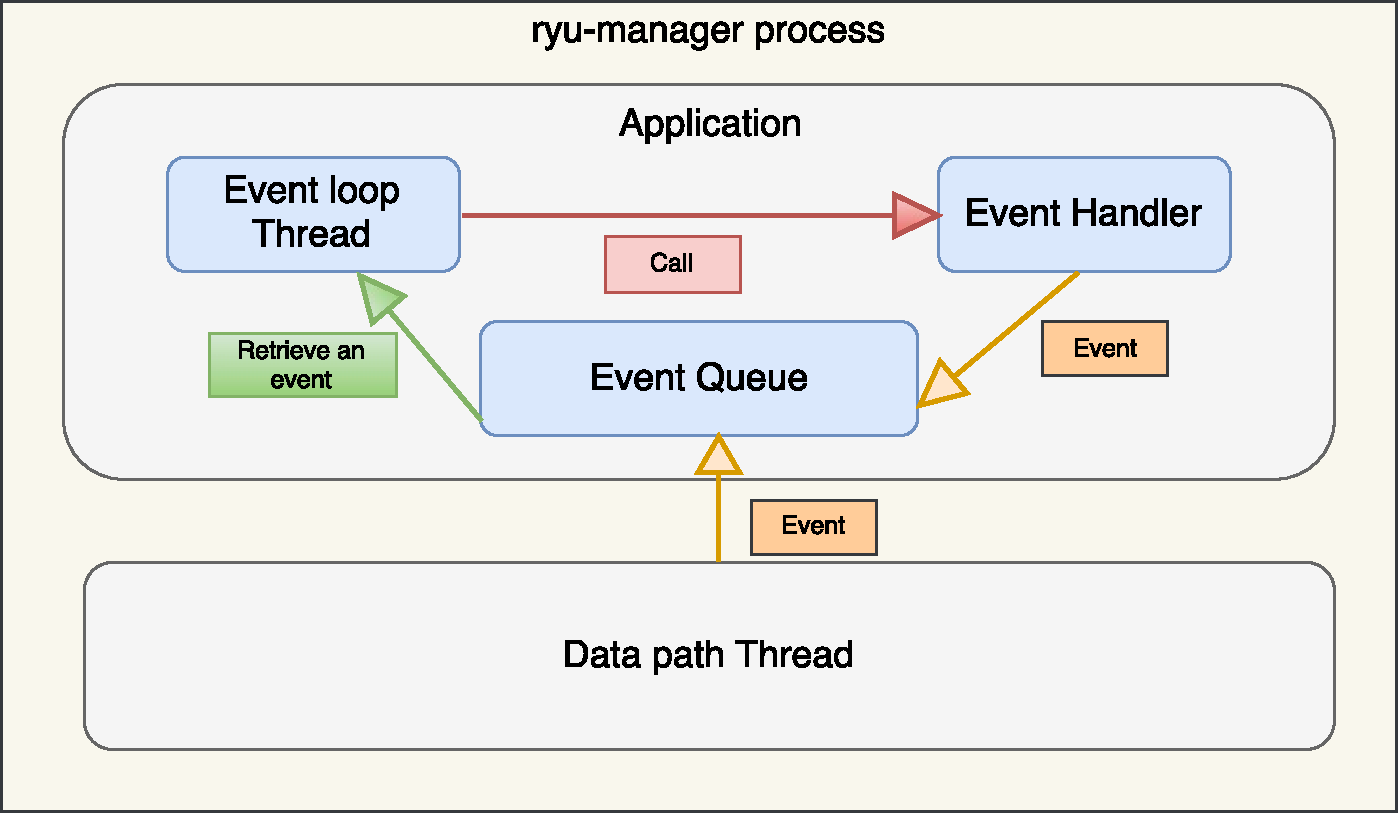
\includegraphics{ryu-architecture.pdf}}
		\caption{Ryu application programming model.}
		\label{fig:ryuarch}
	\end{center}
\end{figure}

\paragraph{Applications:}
Applications are a subclass of \textit{ryu.base.app\_manager.RyuApp}. Ryu applications are single-threaded entities which implement various functionalities in Ryu. User logic is supposed to be implemented as an application.
\paragraph{Event:}
Ryu applications communicate between them, transmitting and receiving events. Events are the objects of a class that inherits \textit{ryu.controller.event.EventBase}. Ryu events can also contain arbitrary python objects.
\paragraph{Event Queue:}
Each Ryu application has a receive queue for receiving events. The queue is implemented as FIFO and retains the order of events.
\paragraph{Event Loop Thread:}
Ryu application runs a thread for event processing from the event queue. The thread runs a loop whenever there is an event available in the queue. The event loop will load the events and will call the appropriate event handler for processing the event type.
\paragraph{Datapath Thread:}
Datapath thread is used to describe the connection of the OpenFlow switch with a controller. It is an instance of the class \textit{ryu.controller.controller.Datapath}. Threads and queues in Ryu are implemented with python eventlet/greenlet package.
\paragraph{Event Handlers:}
An event handler is a method in the user application class using the decorator \textit{ryu.controller.handler.set\_ev\_cls}. Application events loop queued events from the event queue and the defined event handler is called.
\paragraph{ryu-manager:}
This is the main executable to start a Ryu application. It instantiates the single instance of class \textit{ryu.base.app\_manager.AppManager}. This internally loads Ryu applications, create contexts to Ryu applications, and start the services.

\subsection{Iperf and Socat}
Iperf is a tool normally used for measuring the throughput of the network. It can create Transmission Control Protocol (TCP) and User Datagram Protocol (UDP) data streams, which are used to measure the throughput. It is developed in C and has both client (to generate traffic) and server (to discard traffic) functionality and able to measure throughput between any connected two ends of network unidirectionally or bi-directionally. It can generate controlled traffic (UDP mode) for a specified duration. It is an open source, cross-platform tool and can be used for both wired and wireless networking equipment testing \cite{iperf}. Iperf supports various parameters for testing a network, or for optimizing or tuning a network. The controlled data stream generation functionality of iperf is used for generating traffic in the emulation testbed (see Figure \ref{fig:emulator}) \cite{iperfman}.

Socat is a command line based powerful utility with many features. It can establish two bidirectional byte stream for reading or writing data between two ends. It can be used for almost any kind of data transferring between any kind of stream. Socat supports a various feature like redirection of TCP, UDP, and SCTP ports to other sites; execution of commands; start a child process and much more, it is a Switch knife for the user. It is used as a data sink in the CA for receiving data along with its child process creation facility to resend the received packet back to the data source (see Figure \ref{fig:emulator}) \cite{socatman}.

\subsection{Tc and NetEm} \label{sec:tan}
Tc is used to configure Traffic Control in the Linux kernel. Traffic Control is used to specify the sets of queuing systems and mechanisms by which packets are received and transmitted in the network. Its functionality can be used in deciding which packet to accept or transmit, in what order, and at what rate on the input or output of a network interface \cite{howtc}. This section of description is mainly based on the tc and netem man page \cite{tc-man} \cite{netemman}. Traffic Control consists of the following operations:

\begin{itemize}
	\item SHAPING, to control the rate of egress traffic.
	\item SCHEDULING, to improve the interactivity for egress traffic.
	\item POLICING, to limit the ingress traffic as opposed to shaping.
	\item DROPPING, to discard both on ingress and on egress.
\end{itemize}

The processing of traffic is controlled by three kinds of objects: qdiscs, classes, and filters.
\paragraph{QDISCS:} Qdisc is an abbreviation for `queueing discipline'. Kernel always enqueues packets to the qdisc configured for an interface to send a packet to it. There are two types of qdiscs. One is the classful qdiscs (e.g., pfifo, bfifo, pfifo\_fast, red, sfq, tbf), which can contain classes and provide a handle to attach filters. Another is the classless qdiscs (e.g., CBQ, HTB, PRIO) which do not contain classes, making it impossible to attach a filter. Normally, the simple classful qdisc pfifo, which does no processing at all and is a pure First In, First Out queue, is the default.
\paragraph{CLASSES:} Classful qdiscs can contain classes, which contain further qdiscs. Traffic may then be enqueued in any of the inner qdiscs, which are within the classes.
\paragraph{FILTERS:} A filter is used by a classful qdisc to determine in which class a packet will be enqueued. On the arrival of traffic, it needs to be classified and the filter is one method to classify it. Filters reside within qdiscs and does not govern any event. All filters attached to the class are called until one of them returns with a match.

While in operation, classes form a tree and each class has a single parent. A class may have multiple children. Qdiscs CBQ, and HTB allow for runtime addition of classes while PRIO is created with a static number of children. Qdiscs, which allow dynamic addition of classes, can have zero or more subclasses to which traffic may be enqueued. Furthermore, each class contains a leaf qdisc which by default has pfifo behavior, although another qdisc can be attached in place. When a packet enters a classful qdisc, it can be classified based on three criteria (i.e., tc filter, Type of Service, and skb-priority) to one of the classes within. Each node within the tree can have its own filter, but higher level filters may also point directly to lower classes. If classification does not succeed, packets are enqueued to the leaf qdisc attached to that class.

NetEm is an enhancement of the Linux traffic control facility that allows adding delay, packet loss, duplication, and other characteristics to packets outgoing from a selected network interface. NetEm is built using the existing Quality Of Service (QOS) and Differentiated Services (diffserv) facilities in the Linux kernel.

For the purpose of this study, Linux Traffic Control functionality with NetEm (to add delay) for emulating the processing capability in CAs is used. Its implementation is further discussed in Section \ref{sec:tmfg}. 